\section{NAT}

\begin{bonus}{Konfiguration von IPv4-Adressen}
    \emph{IPv4-Adressen} müssen in jedem Endgerät, Router und sonstigen Netzwerkkomponenten konfiguriert werden.

    Jeder Knoten muss folgende Daten besitzen:
    \begin{itemize}
        \item IP und Netzwerkmaske
        \item Standard-Gateway
        \item DNS-Server
    \end{itemize}

    Grundsätzlich existieren zwei Möglichkeiten dazu:
    \begin{itemize}
        \item Manuelle Konfiguration
        \item Konfiguration über ein Protokoll (z. B. DHCP)
    \end{itemize}
\end{bonus}

\begin{bonus}{Probleme IPv4}
    Wir hatten bereits geklärt, dass IPv4 nur $2^{32}$ IP-Adressen zur Verfügung hat.

    Da bereits relativ zeitnah nach dem Anpassen der Subnetzgrößen klar wurde, dass die gewonnene Anzahl der daraus resultieren IP-Adressen nicht ausreicht, hat man sich eine provisorische Lösung überlegt.
\end{bonus}

\begin{defi}{NAT}
    \emph{NAT} (Network Adress Translation) verfolgt die Idee, dass KundInnen jeweils lediglich eine eindeutige öffentliche IPv4-Adresse erhalten.
    Dementsprechend existiert für jedes Netz ebenfalls nur einen Zugangspunkt (Gateway) zu diesem Netz.
    Das Gateway hat dabei mindestens 2 Netzwerkkarten, um in das große Internet, sowie das lokale Netz zu senden.

    Das private Netz hat nutzt meist einen der folgenden IP-Adressblöcke:\\
    \begin{tabular}{llcl}
        \texttt{10.0.0.0/8:}     & \texttt{10.0.0.0}    & - & \texttt{10.255.255.255}  \\
        \texttt{172.16.0.0/12:}  & \texttt{172.16.0.0}  & - & \texttt{172.31.255.255}  \\
        \texttt{192.168.0.0/16:} & \texttt{192.168.0.0} & - & \texttt{192.168.255.255}
    \end{tabular}
\end{defi}

\begin{example}{NAT}
    \begin{center}
        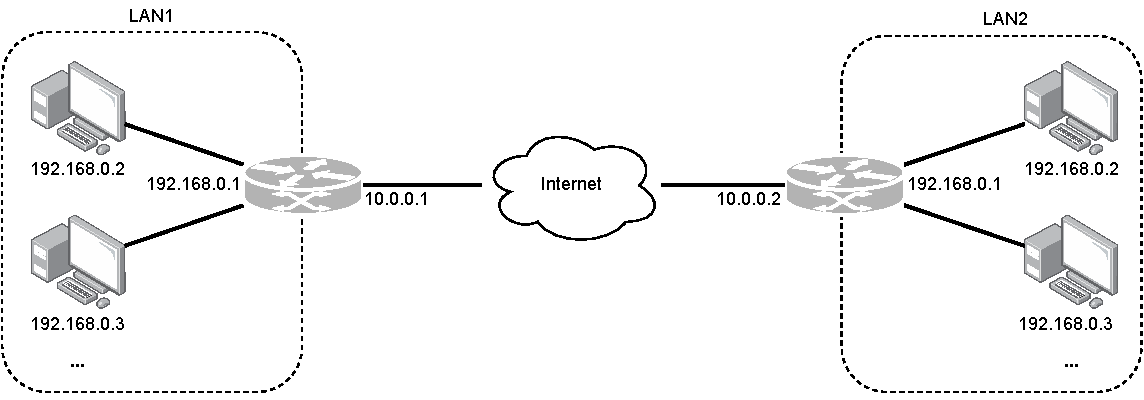
\includegraphics[width=0.75\textwidth]{includes/figures/defi_nat.pdf}
    \end{center}

    In diesem Beispiel \enquote{verbrauchen} wir 2 globale IP-Adressen, können jedoch bis zu $(2^{16} - 3)$ Adressen in jeweils 2 Netzen anbinden.
\end{example}

\begin{defi}{Adressübersetzung (NAT)}
    Zur Identifikation des Absenders bzw. Empfängers müssen im IP-Header freie Felder gefunden werden.
    Im IP-Header steht jedoch nur noch 1 freies Bit zur Verfügung.

    \begin{center}
        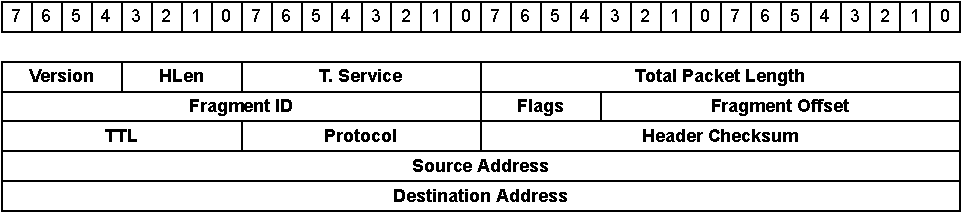
\includegraphics[width=0.75\textwidth]{includes/figures/defi_ip_header.pdf}
    \end{center}

    Zweite Idee: Nutze TCP bzw UDP Header.
    Hier kann man die 16 bit Portnummern nutzen um Clients eindeutig zu Adressieren.
    Hierbei wird jedoch die Schichten Architektur verletzt, da Layer 3 Details über Layer 4 hat.

    \begin{center}
        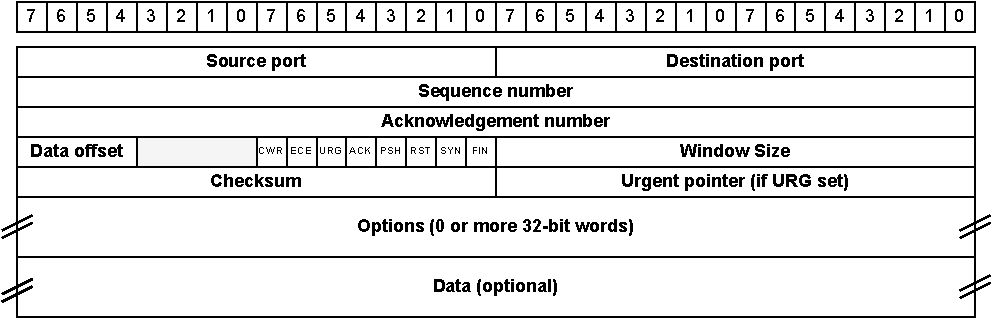
\includegraphics[width=0.75\textwidth]{includes/figures/defi_tcp_header.pdf}
    \end{center}
\end{defi}